\section{Examples previously seen in book}
\subsection{Equivalence Relation as a Category}
\begin{proofitem}
    \item
\begin{align}
    x \in S \implies (x, x) \in S &&\text{reflexivity}\\
    (x,y) \in R \implies (y, x) \in R &&\text{symmetry}\\
    (x,y) \land (y, z) \in R \implies (x, z) \in R &&\text{transitivity}
\end{align}
\item
Categories can be seen to be inspired by equivalence relations. Start with a set
$S$ that has an equivalence relation $R$.
\begin{enumerate}
    \item Objects: $x\in S$.
    \item Arrows: $x\in R\subseteq S\times S$.
\end{enumerate}
\item Let $\mathcal{C}_{\text{eq}}$ be the category formed from an equivalence
    relation.
\item To show that $R$ and $S$ form a category, we must show that it adheres to
    the two required properties of categories: unit laws and associativity.
\item The unit laws requires that for any arrow $f:a \rightarrow b$, there
    exists arrows $1_a \land 1_b$ such $f\circ 1_a = f = 1_b \circ f$.
\begin{figure}[H]
\begin{align*}
    f\circ 1_a=& (a, b)\circ (a, a)&\exists(a,a)\text{ from reflexivity}\\
    =&(a, b)\\
    =&f\\
    1_b\circ f=& (b, b)\circ (a, b) &\exists(b,b)\text{ from reflexivity}\\
    =&(a, b)\\
    =&f
\end{align*}
\caption{Unital Laws}
\end{figure}
\item Thus we have shown the category $\mathcal{C}_{\text{eq}}$ adheres to the unital laws.
\item The associativity laws requires that for arrows $f, g, h,
        a \overset{f}{\rightarrow} b \overset{g}{\rightarrow} c
        \overset{h}{\rightarrow} d, (h\circ g)\circ f=h\circ (g \circ f)$.
\begin{figure}[H]
\begin{align*}
    (h\circ g)\circ f=&((c, d)\circ (b, c))\circ (a, b)\\
    =&(b, d)\circ (a, b)&\text{via transitivity}\\
    =&(a, d)\\
    h\circ (g\circ f)=&(c, d)\circ ((b, c))\circ (a, b))\\
    =&(c, d)\circ (a, c)&\text{via transitivity}\\
    =&(a, d)
\end{align*}
\caption{Associative Laws}
\end{figure}
\item Thus we have shown the category $\mathcal{C}_{\text{eq}}$ adheres to the
    associative laws.
\item Conversely, can you put some conditions on a category to ensure that it
    “is” an equivalence relation?
\item To assure that some category $\mathcal{C}$ forms an equivalence relation,
    we must assure that that $\mathcal{C}$ gives rise to three properties
    required for an equivalence relation: reflexivity, symmetry, and
    transitivity. Reflexivity and transitivity are guaranteed for any category
    via the unital and associative properties---requirements to be a category. To
    satisfy symmetry, for any arrow $f:a\rightarrow b\in \mathcal{C}$, there
    must exist an arrow $g:b\rightarrow a\in \mathcal{C}$.

    Additionally, there can be only arrow between any two objects $a, b \in
    \mathcal{C}$. This uniqueness property between two objects is required
    because a relation $R$ is a set, and a set is defined by some characteristic
    function, which is a function with a boolean codomain. Either an element is
    in or out of the set, and more than one arrow between the same objects would
    violate this requirement.
\end{proofitem}

\begin{table}
    \centering % Optional, for centering the table
    \begin{tabular}{ ccccc } % 5 columns, each centered
    \hline
    & Equivalence Relation & & Category & \\ \hline
    Data & objects & $\rightarrow$ & objects& Data\\
    Structure & relations & $\rightarrow$ & arrows & \\ \hline
    & reflexivity & $\rightarrow$ & identities & \\
    Properties & symmetry & $\rightarrow$ & inverses & Structure \\
    & transitivity & $\rightarrow$ & composition & \\\hline
    & & & unit laws& Properties \\
    & & & associativity &
    \\\hline
    \end{tabular}
    \caption{Properties become structure, and a new layer of properties is required.}
\end{table}
\subsection{Factors of $n\in\mathbb{N}$ as a Category}
Pick a number. The objects are the factors, and the arrows $a\rightarrow b$ are
whenever a is a factor of $b$. In this cateogry, like the equivalence-relation
category, there is at most one arrow between two objects. That is because this
category is again representing a relation. Any relation $(a, b)$ can only be in
a set once, per the definition of set.
\begin{figure}[H]
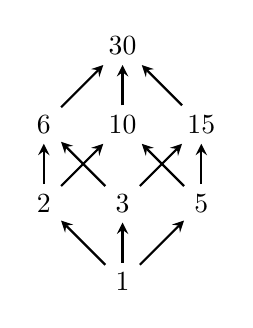
\begin{tikzpicture}[->, >=stealth, thick]
\node (1) at (2,0) {$1$};
\node (2) at (1,1) {$2$};
\node (3) at (2,1) {$3$};
\node (5) at (3,1) {$5$};
\node (6) at (1,2) {$6$};
\node (10) at (2,2) {$10$};
\node (15) at (3,2) {$15$};
\node (30) at (2,3) {$30$};
\draw (1) -- (2);
\draw (1) -- (3);
\draw (1) -- (5);
\draw (2) -- (6);
\draw (2) -- (10);
\draw (3) -- (6);
\draw (3) -- (15);
\draw (5) -- (10);
\draw (5) -- (15);
\draw (6) -- (30);
\draw (10) -- (30);
\draw (15) -- (30);
\end{tikzpicture}
\caption{30-factor Category}
\end{figure}
\subsection{Factors of $\mathbb{N}$ as a Category}
If we took all of $\mathbb{N}$ as a category, then there would be a morphism
from $0$ to all other objects, except itself. In fact, $0$ couldn't be in the
category, because there couldn't be an identity relation as $\frac{0}{0}$ is
undefined. If we modify the set to be $\mathbb{N} - \set{0}$, then there would
be a morphism from $1$ to all other elements. Each prime number would have two
morphisms---the identity morphism and one from $1$ to itself.
